\chapter{Paper III}\label{chap:paper3}
\section{Introduction}\label{sec:p3-intro}
Following on from the previous paper, we wished to apply our implemented MPLE on other interesting subsamples of the \textit{Gaia} data. We were also able to make use of the improved Gaia DR3. 

The study of kinematic space has a division in it between the Galactic disc and the stellar halo. This division guides our choice of samples and is understandable since the two regions are affected by different dynamical processes. The disc we have already described in section \ref{sec:p2-intro}. The stellar halo on the other hand, is where the evidence of past mergers between the Galaxy and its neighbours will be found \citep{helmi:20}, which can, for example, contribute to the velocity distribution and cause enhanced star formation \citep{ruiz-lara:20}. This is what inspires our chosen samples of data: the Solar neighbourhood disc sample and a the stellar halo.

Since our method lets us utilise the astrometry only, we can then achieve some impressive sets of data for these populations. Limiting the Solar neighbourhood to $\varpi > 5$ mas (or 200 pc) we can use as many as 1 171 846 stars, after having applied all of our quality cuts. This is comparable to current results using the Gaia RVS like \cite{lucchini:22} which has 982 879 stars in the Solar neighbourhood. However, they do not apply any quality filters on photometry or astrometry, apart from a criteria of 20\% parallax uncertainty $(\varpi / \sigma_\varpi > 5)$. We restrict our results to only 10\% uncertainty and if we were to use 20\%, we would have 3 592 434 sources before applying our quality filters, which highlights the benefits of our method.

For the stellar halo, a recent similar sample is \cite{dodd:22} which limits their halo to 2.5 kpc as well as imposing a velocity cut whereby the motions of the star with respect to the Local Standard of Rest (LSR) must be greater than 210 km/s. Since the circular speed at the position of the sun is ${\sim}$233 km s$^{-1}$ \citep{mcmillan:17}, this cut removes the vast majority of the disc stars. Our cuts are slightly more generous with a distance limit of 3 kpc and velocity limit of at least 200 km s$^{-1}$, albeit on transverse velocity rather than full space velocity. Their sample contains 72 274 stars, whereas ours contains 456 273. 

We use these two samples to estimate their velocity distributions. For the Solar neighbourhood, this is done in the same manner as for the WDs in the previous paper. The stellar halo distribution is inferred in spherical coordinates instead, since it is more spherical in shape around Galaxy. We also divide the stellar halo into \textit{in situ} and \textit{accreted} components (e.g., \citealt{naidu:20}). The velocity distributions are studied closely to determine what known structure is apparent and what new structure we are able to identify. Some novel structures do appear in our analysis, specifically in the accreted halo where we find two new features that we call \textit{MMH-1} and \textit{MMH-2}.
\section{Gaia's view of the local Galaxy}\label{sec:p3-gaiaview}
\begin{figure}[t]
    \centering
    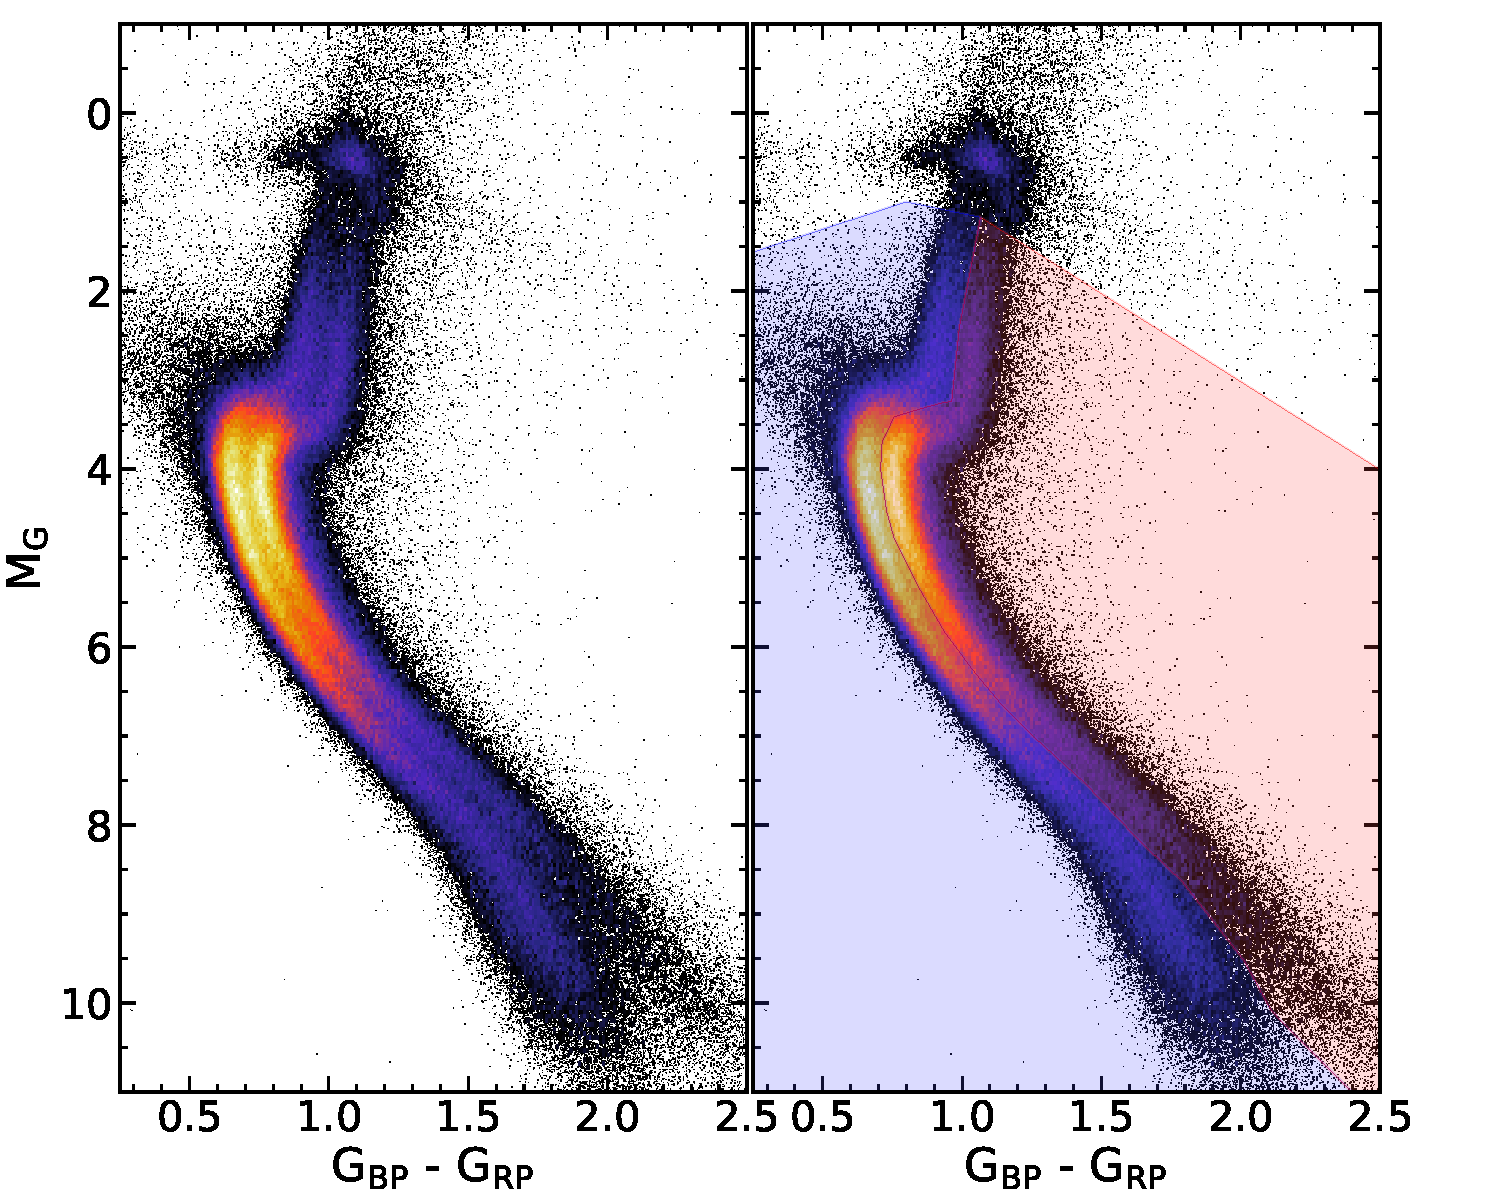
\includegraphics[width=0.75\textwidth]{images/GES_cmd.pdf}
    \caption{Colour-magnitude diagram of our filtered halo sample. Colour shows the number density. Right panel shows selected regions for the left and right sequences overlaid with shaded areas.} % Fig. 5.1
    \label{fig:halo_cmd}
\end{figure}
\begin{figure}[t]
    \centering
    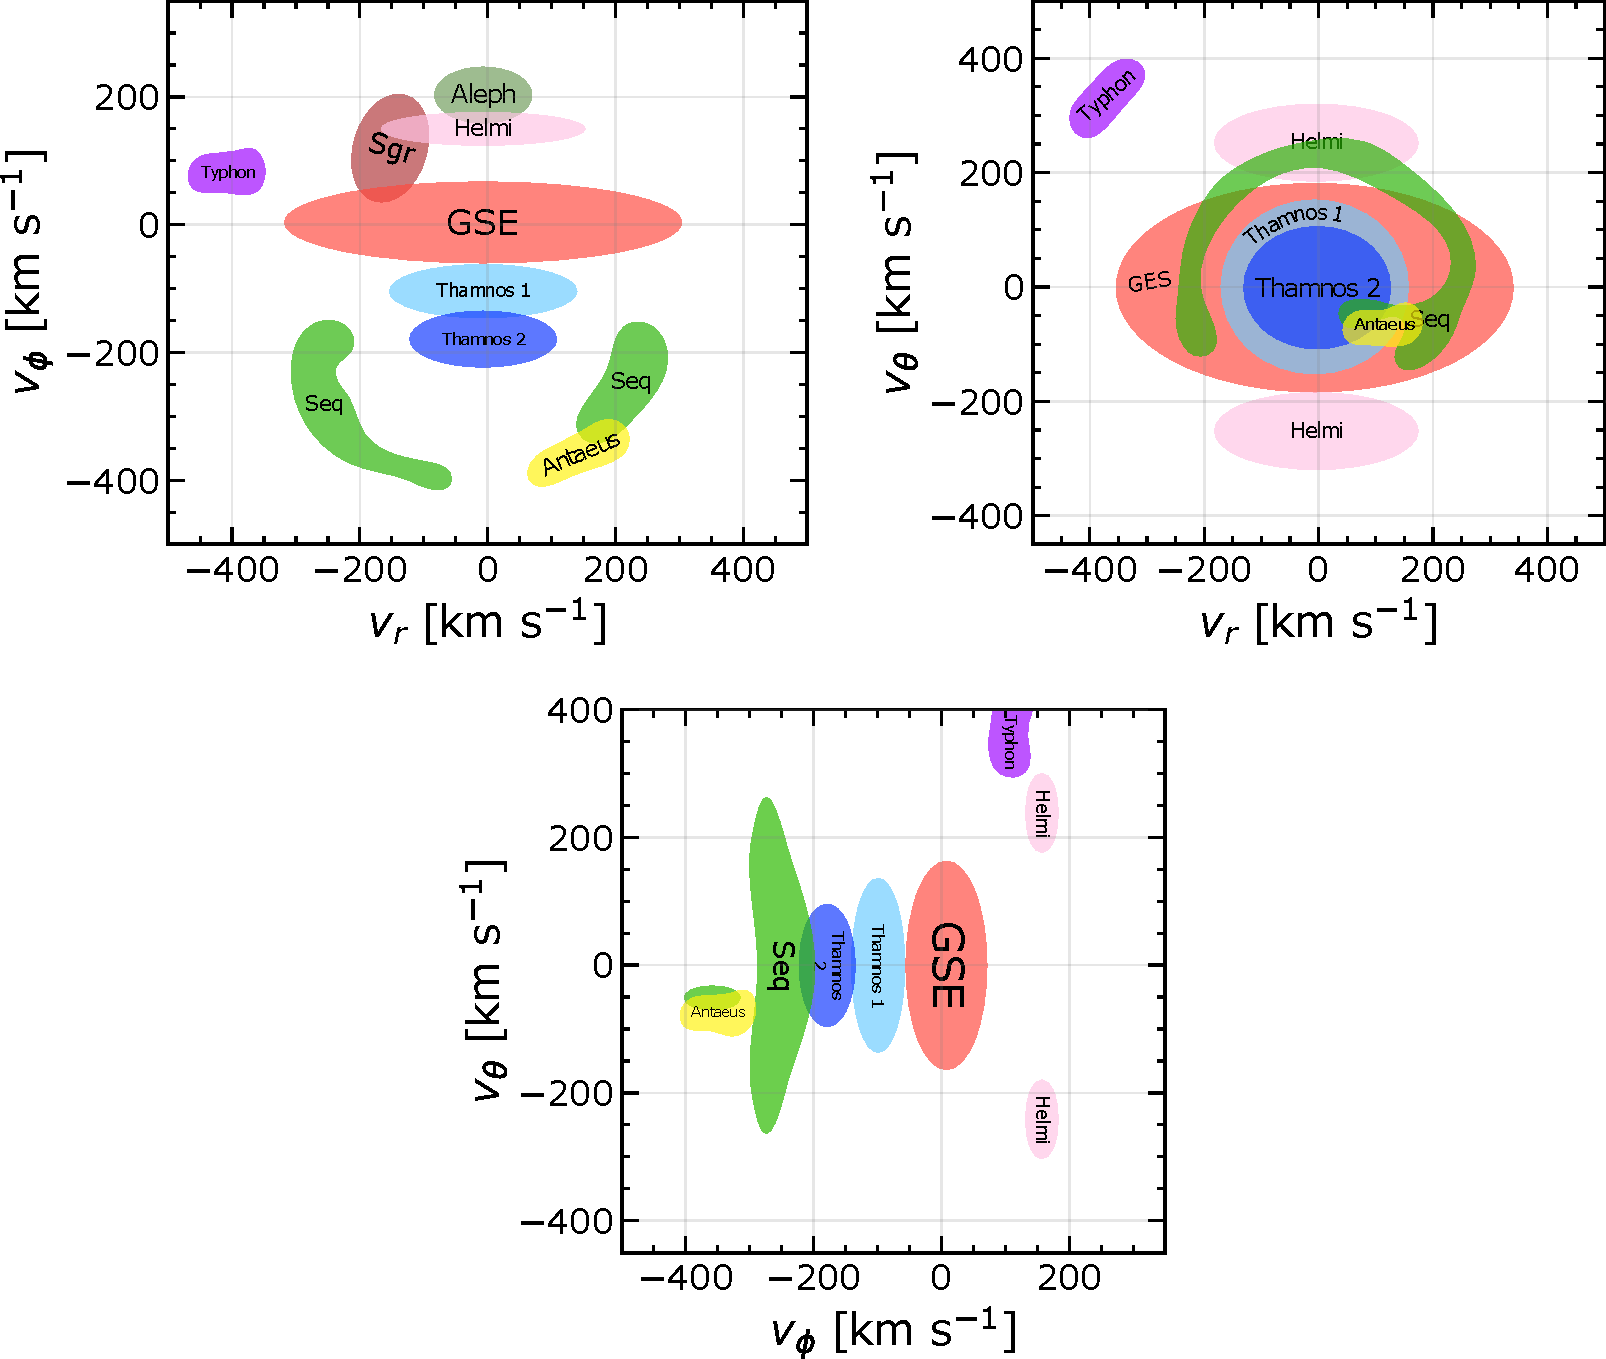
\includegraphics[width=0.85\textwidth]{images/map_only_b.pdf}
    \caption{Estimated typical positions of known velocity structures in the stellar halo. Figures show the velocity spaces of $(v_r, v_\phi)$ (top left), $(v_r, v_\theta)$ (top right), and $(v_\phi, v_\theta$ (bottom). Here $v_r$ points outwards from the Galactic centre, $v_phi$ increases in the direction of Galactic rotation, and $v_\theta$ increases from south to north Galactic poles.} % Fig. 5.2
    \label{fig:halo_map}
\end{figure}
There has been plenty of work done to try and characterise the velocity substructure that exists in the disc and stellar halo. We briefly discussed the Solar neighbourhood in chapter \ref{chap:paper2} and showed several moving groups from \cite{antoja:12} in Fig. \ref{fig:wd_fv}. We briefly mentioned \cite{lucchini:22} above which is one of the more recent works that investigates the disc structure. The current picture of the local disc velocity distribution is one with multiple arch-like structures, of which many fractured individual substructures can be identified (see e.g., Table 1 from \citealt{lucchini:22}). 

For the stellar halo, things look slightly different. This is currently a very active field, but some smaller discoveries were made already 20 years ago using Hipparcos to identify the Helmi streams \citep{helmi:99}. It is, perhaps, not surprising that \textit{Gaia} has had a significant impact upon this field as well. When DR2 was released, two important findings came soon thereafter. The first was in the colour-magnitude diagram of the stars with large transverse velocities. By selecting stars with $v_T > 200$ km s$^{-1}$ \cite{dr2:hr} showed that there were two separate main sequences, a finding that we recreate and show in Fig. \ref{fig:halo_cmd}. The left sequence was then found to be connected to an accretion event from a single object \citep{belokurov:18, koppelman:18} which is called \textit{Gaia-Sausage-Enceladus} or \textit{GSE}, which was the second finding. This lead to a successful hunt for other accreted populations in the stellar halo. At the time of writing, some of the larger discovered structures include \textit{Sequoia} \citep{myeong:19}, \textit{Antaeus} \citep{oria:22}, \textit{Thamnos} 1 and 2 \citep{koppelman:19}, and \textit{Typhon} \citep{tenachi:22}, to name a few. We show the expected positions of these features as well as some smaller ones in Fig. \ref{fig:halo_map}. This puts into perspective how structured the Galactic stellar halo has been revealed to be with the use of \textit{Gaia} data.

Since we have access to the most expansive catalogue of sources from \textit{Gaia}, we aim to expand the view of substructure in the local parts of the Galaxy's disc and stellar halo.

\section{Structures: The old and the new}\label{sec:p3-structures}
\begin{figure}[t!]
    \centering
    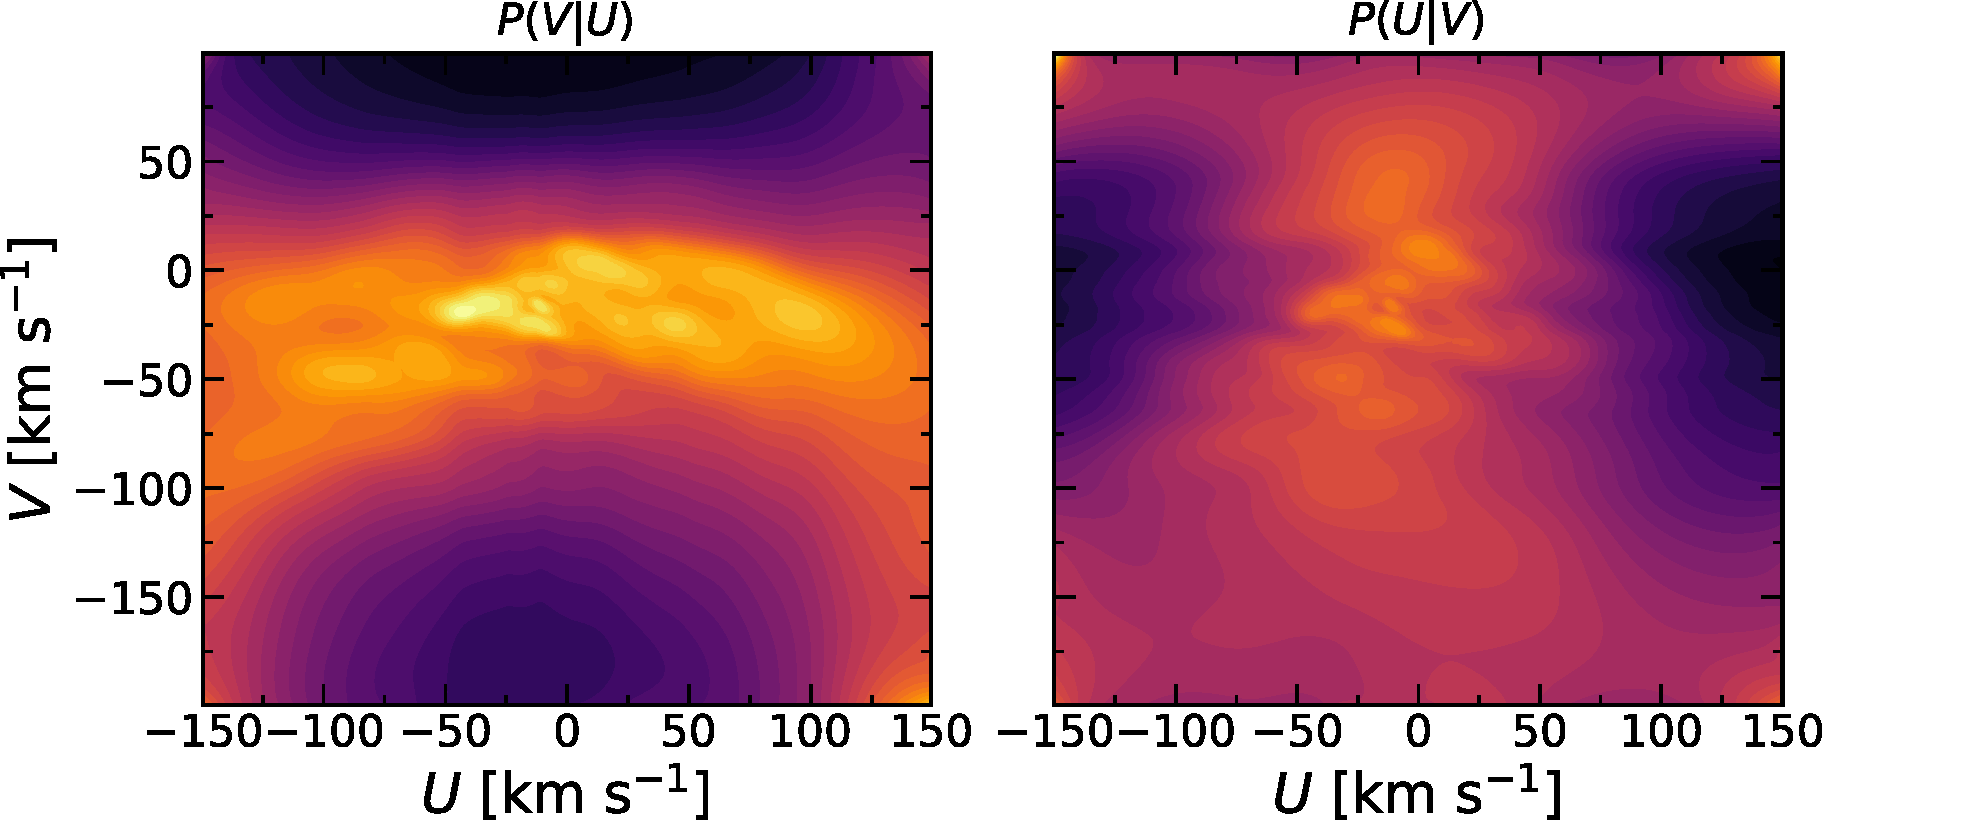
\includegraphics[width=0.9\textwidth]{images/conditional_snbh.pdf}
    \caption{The conditional probability of one velocity component in $(U, V)$ against the other. Left shows $P(V|U)$ and right shows $P(U|V)$ which reveals rich substructure beyond the central dominating groups. The color scaling shows the density such that $P(v)^{0.25}$.} % Fig. 5.3
    \label{fig:cond_snbh}
\end{figure}
\begin{figure}[t!]
    \centering
    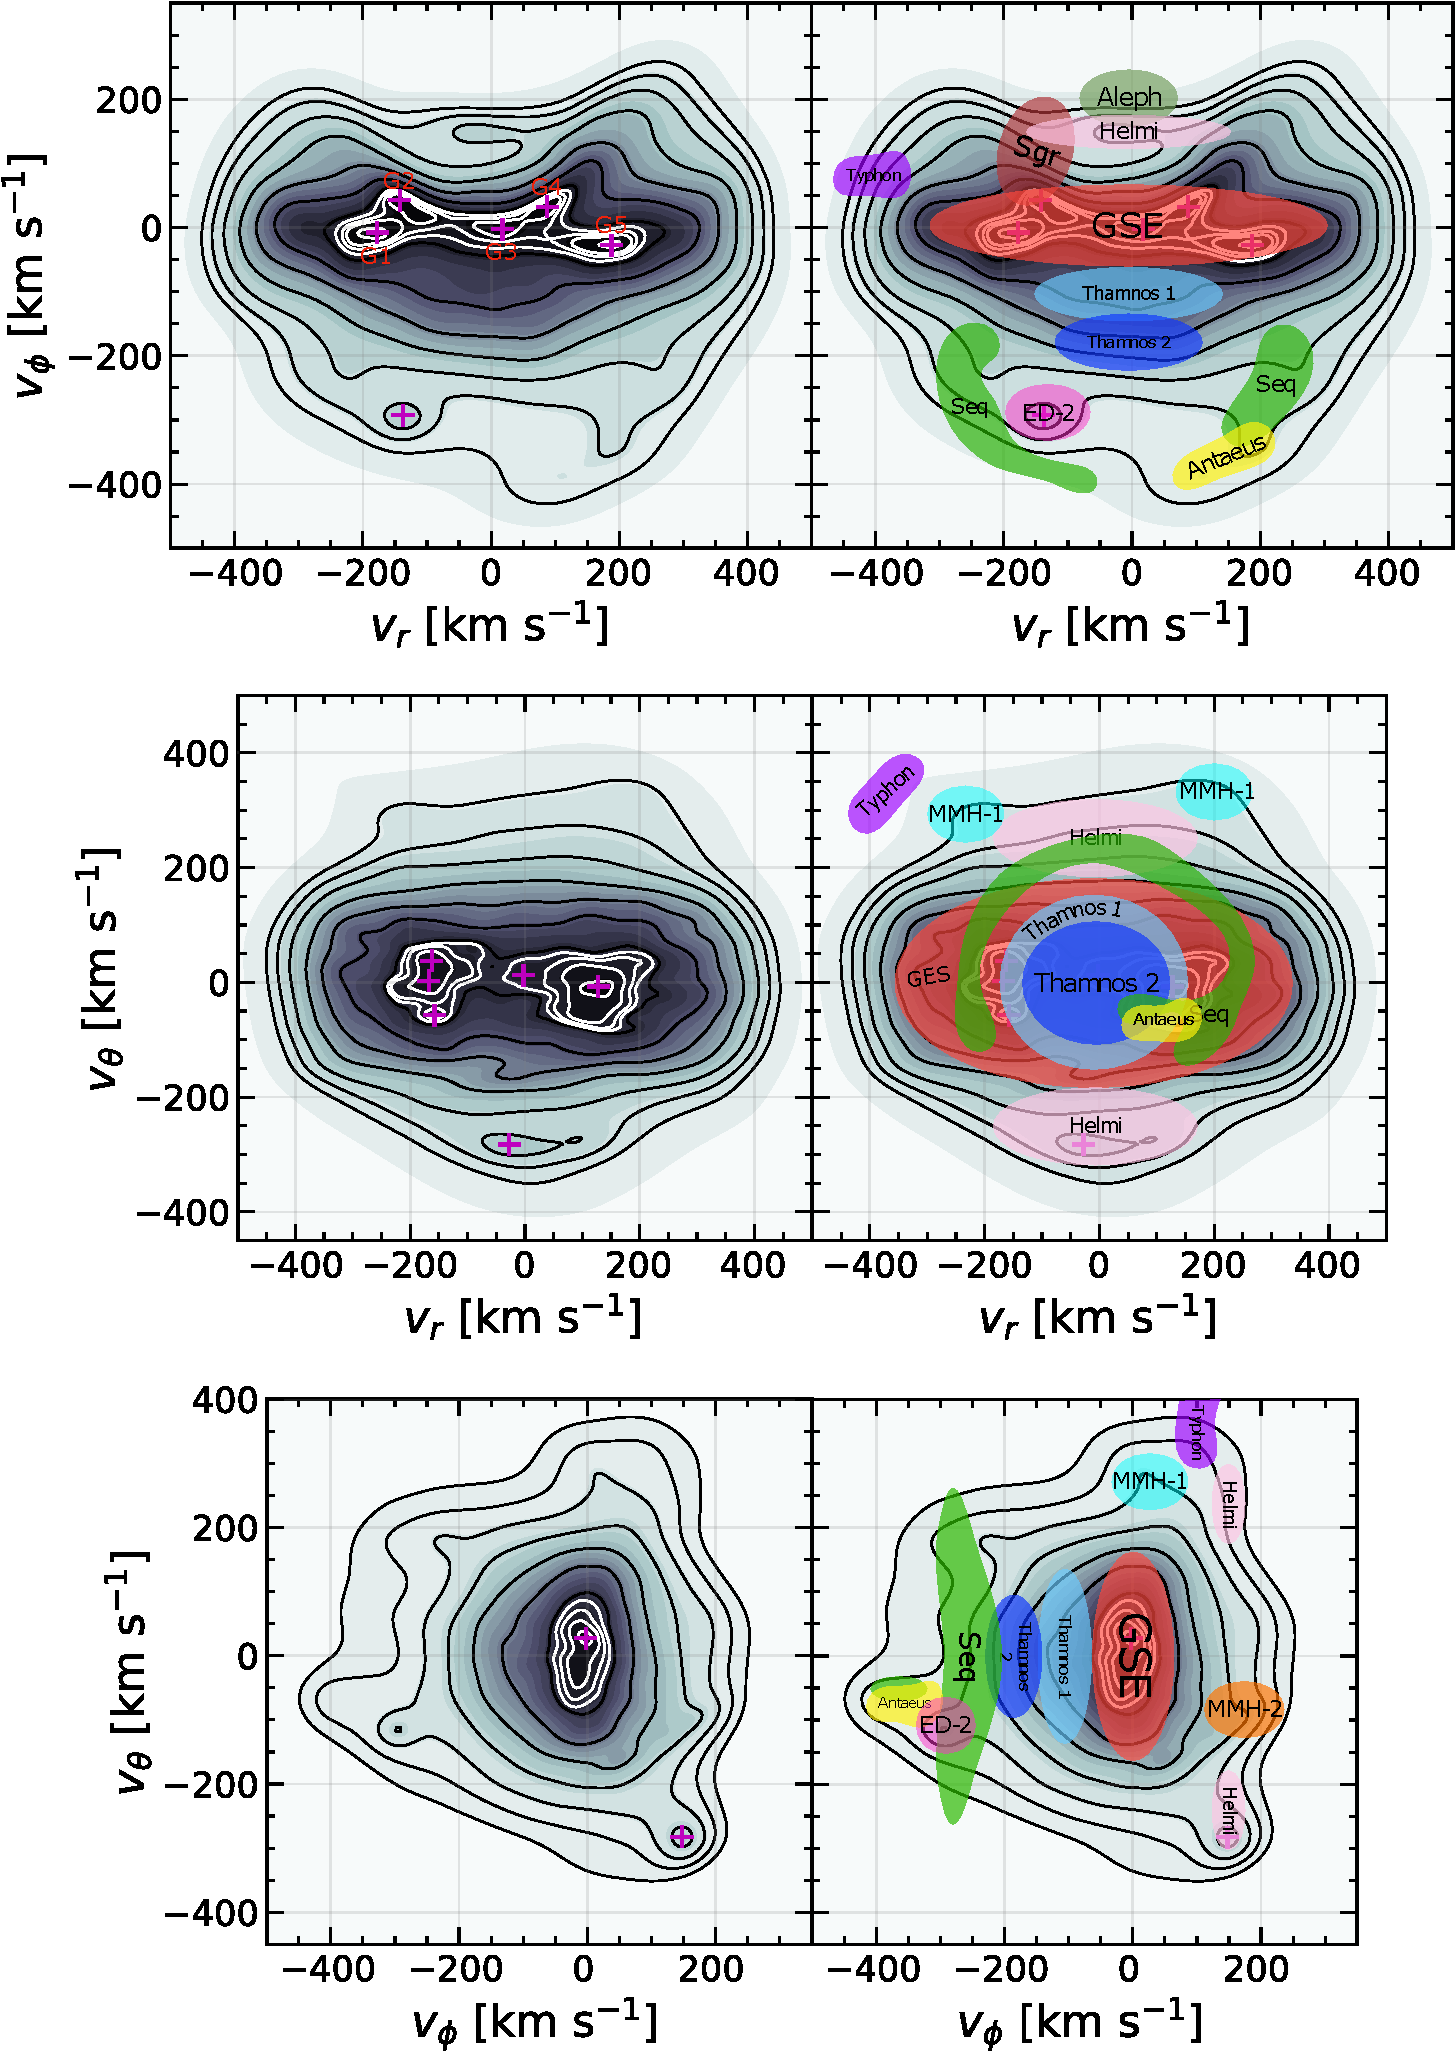
\includegraphics[width=0.8\textwidth]{images/halo_fv.pdf}
    \caption{Velocity distributions of our left halo sample in $(v_r, v_\phi)$ (top row), $(v_r, v_\theta)$ (middle row), and $(v_\phi, v_\theta$ (bottom row). Right right column shows the same distributions overlaid with the positions of expected substructure from literature, in a similar style to what is done in \cite{naidu:20} and \cite{mardini:2022}. Significant peaks are marked with purple crosses and in the top left figure five significant groups belonging to the \textit{GSE} are marked as G1-G5.} % Fig. 5.4
    \label{fig:halo_fv}
\end{figure}
\begin{figure}[t!]
    \centering
    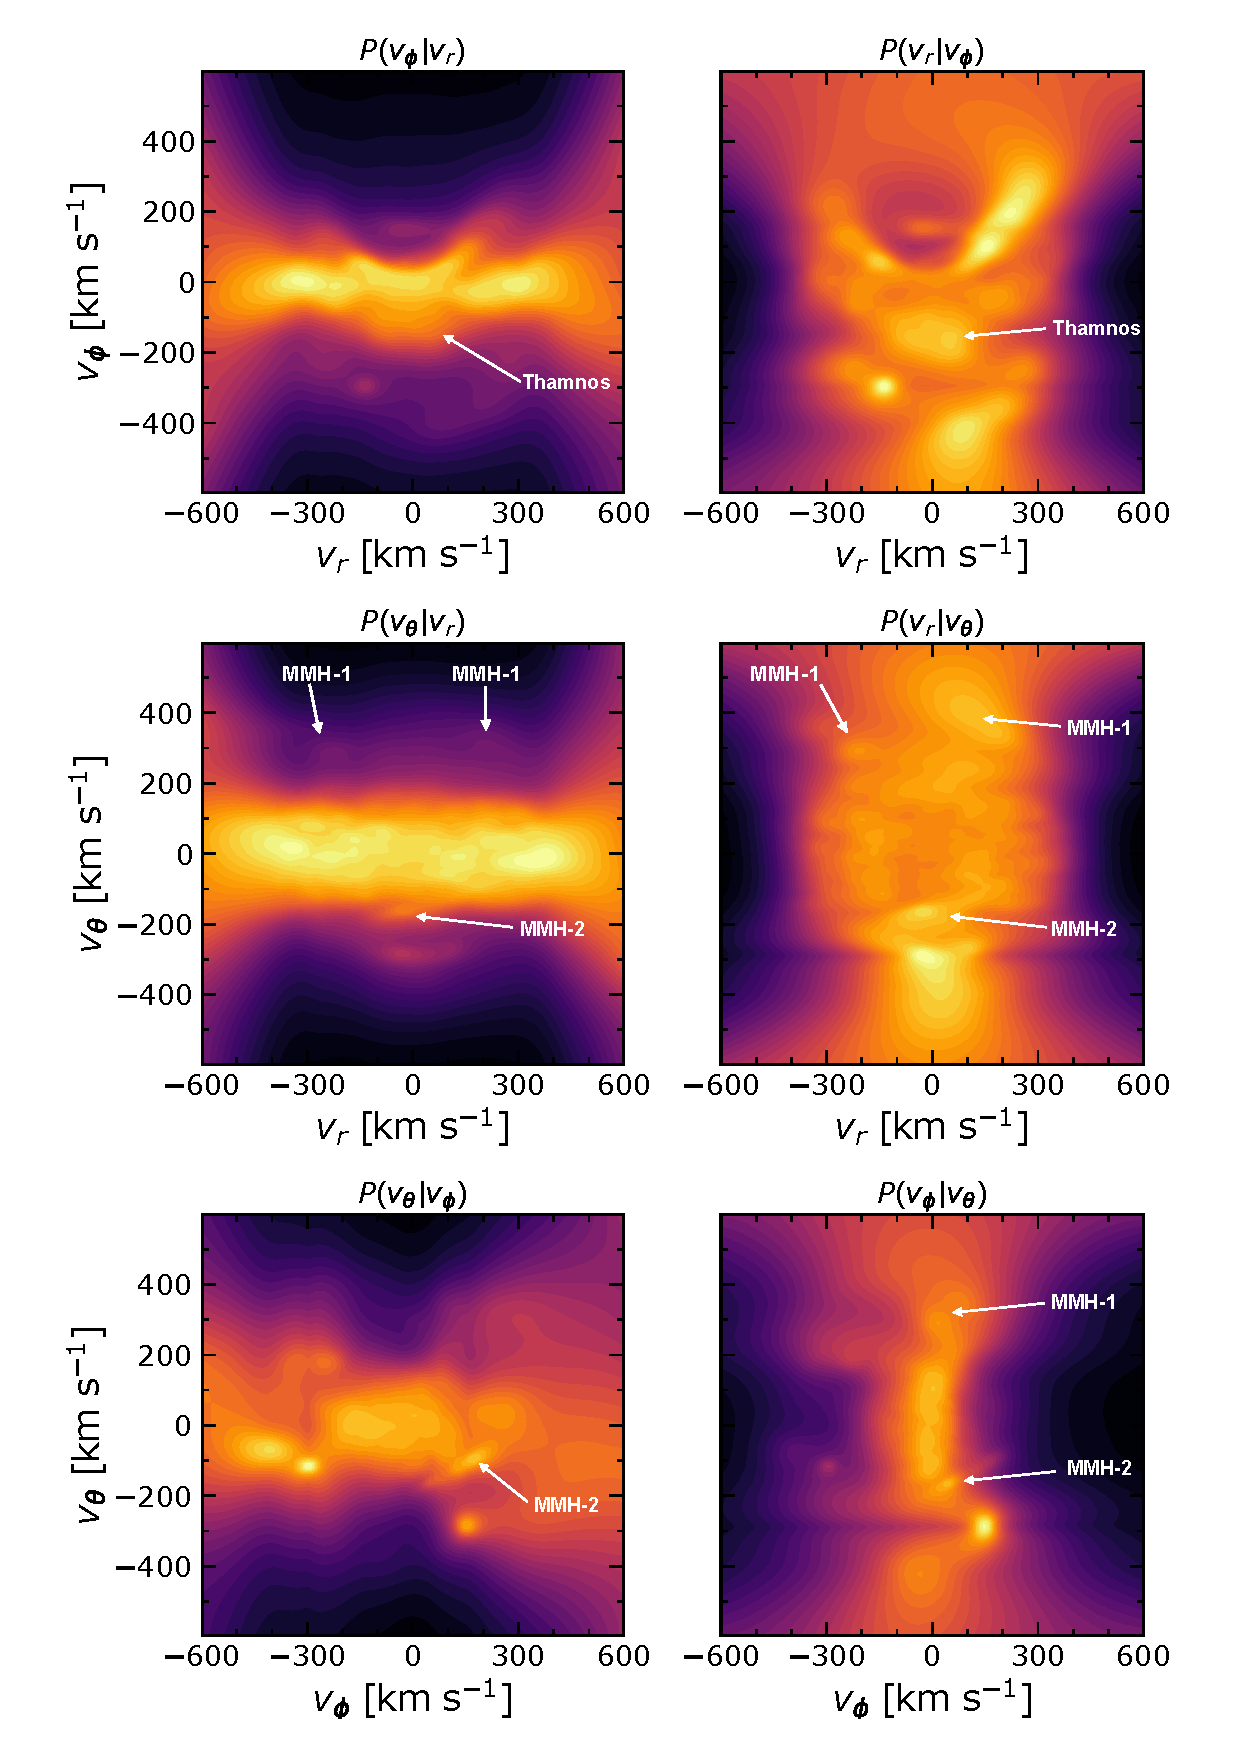
\includegraphics[width=0.8\textwidth]{images/conditional_halo.pdf}
    \caption{Conditional probability distributions of the velocities from Fig. \ref{fig:halo_fv} with the left column showing the conditional probability distribution of the $y$-axis velocity on the $x$-axis velocity. The right column shows the inverted conditional probabilities. Density is scaled such that $P(v)^{0.25}$.} % Fig. 5.5
    \label{fig:cond_halo}
\end{figure}
When we investigated the velocity distribution of the Solar neighbourhood using our sample we found that the distribution is heavily dominated by the typical major moving groups: \textit{Sirius}, \textit{Coma Berencies}, \textit{Hyades}, \textit{Pleiades}, and \textit{Hercules}. The distributions also contains weaker traces of \textit{Dehnen98} and \textit{Wolf630}. Since the distribution is so heavily dominated by these features, a better way of viewing hidden structures comes in the form of conditional probabilites. For the $(U, V)$ plane where most of the known structure exists, this means that we calculate $P(V|U) = P(U,V) / P(U)$ and $P(U|V) = P(U,V) / P(V)$. The result is probability maps that can reveal structure that is otherwise blotted out by the major groups and we show this in Fig. \ref{fig:cond_snbh}. Here can be seen much richer structure like $\epsilon$\textit{Ind} (e.g., \citealt{antoja:12, kushniruk:17, bobylev:16}) at $(U, V) = (-100, -50)$ km s$^{-1}$, \textit{Dehnen98} \citep{antoja:12} at $(U, V) = (50, -30)$ km s$^{-1}$, and likely \textit{Antoja12} from e.g. \cite{kushniruk:17} at $(U, V) = (100, -30)$ km s$^{-1}$. The conditional probability is clearly a useful tool for the outer regions.

The velocity distributions of the two halo samples were produced and as expected, the right sequence shows very little accreted structure and a such we placed most of our focus on the left sequence. The velocity distributions are shown in Fig. \ref{fig:halo_fv} and are overlaid with the expected positions of stellar halo substructure from Fig. \ref{fig:halo_map}. These distributions show clearly a lot of the known velocity substructures such as \textit{GSE}, \textit{Sequoia}, and the \textit{Helmi} streams. Particularly the \textit{GSE} in $(v_r, v_\phi)$ shows a lot of structure with significant peaks marked as G1-G5. The groups at largest $v_r$, 1 and 5, are placed where the \textit{GSE} is typically associated (e.g., \citealt{feuillet:21}). G2 and G4 lie near the region which is removed by our cut of $v_\mathrm{T} < 200$ km s$^{-1}$ and is therefore probably contaminants from  the disc population. Finally G3 matches with Cluster 3 of \cite{lovdal:22} which is also called \textit{L-RL3} in \cite{dodd:22}. The distributions do show some of the smaller features as well and particularly the low $v_\theta$-component of the \textit{Helmi} stream is very pronounced here. These figures give a good impression of what the accreted stellar halo looks like at `face-value'.

Beyond the known velocity substructure, we can see some additional features. We identified six features not belonging to the larger known groups and they are marked in the figure from 1-6. The strongest of them is Group 1, which is associated with Group 5. We confirmed their association by viewing their respective spaces in slices of the third velocity component. This reveals that Group 1 appears when $v_\theta \in [-200, -100]$ km s$^{-1}$ and Group 5 when $v_r \in [-200, -100]$ km s$^{-1}$, meaning that they share position in 3D velocity space. Comparison with \cite{dodd:22} also shows that they have previously identified this group as \textit{ED-2} and that it occupies about 0.05\% of their sample. This region of velocity space makes up around 0.075\% in our sample, suggesting that the group is slightly larger than previously believed. The same analysis in velocity space let us connect Groups 2, 3, and 6 into a new velocity feature, \textit{MMH-1} which has no prior associations in literature. Lastly, group 4 which we named \textit{MMH-2} was difficult to identify in the other spaces. Its association became clear when we again looked to the conditional probability, seen in Fig. \ref{fig:cond_halo}. Here, the diagonal feature at $(v_r, v_\theta) = (0, -150)$ km s$^{-1}$ stands out even more, and is the representation of \textit{MMH-2} in this space. These maps also reveal some parts of \textit{Thamnos} at $(v_r, v_\phi) = (0, -200)$ km s$^{-1}$ which could previously not be seen. The extended nature of \textit{MMH-1} at $v_\theta = 300$ km s$^{-1}$ is uncovered as well, stretching to even larger values of $v_\theta$ in both $P(v_r|v_\theta)$ and $P(v_\phi|v_\theta)$ and has what appears to be a symmetrical component at large negative $v_\theta$, which if real would likely imply that this feature has considerable vertical action. This view also shows the strength of \textit{MMH-1} as it appears in both $P(v_\theta|v_\phi)$ and $P(v_\phi|v_\theta)$.

The distributions and their results clearly advocate for the benefits of proper-motion limited catalogues. Until such a time that comparative 6D catalogues are available, these types of methods provide the largest possible data sets for kinematic studies. 

